\chapter{Measurement Campaign} \label{ap:b}

This Appendix summarizes the characteristics of the measurement campaign, which was detailed in \cite{Thiago:Characterization} and \cite{thiago:hyb}, performed in some residences in Brazilian urban area of Juiz de Fora city. The statistical analyses of the Brazilian in-home \ac{PLC} and hybrid \ac{PLC}-wireless channels were supported by estimates of the \ac{CFR}, acquired through this measurement campaign. The channels estimation were performed in seven different middle-class residences, some features of these places are summarized in Table \ref{table_ap}. 

The \ac{CFR} measurement setup, used for acquiring the estimations of \ac{PLC} \acp{CFR}, is depicted in Fig. \ref{fig_setup_PLC}. This setup consists of three main components:

\begin{itemize}
	\item Signal generator: Device composed of an arbitrary signal generator board mounted in a rugged computer. A pre-designed sounding sequence is loaded into it and converted to an analog signal to be submitted to the \ac{PLC} channel under analysis.
	\item Data digitizer: Acts as a receiver, measuring the transmitted sounding signal after propagating through the \ac{PLC} Channel, and converts it into a digital representation for the subsequent analysis.
	\item Coupler: Circuitry used to connect both the signal generator and the data digitizer to the \ac{PLC} channel under analysis. The coupler is essentially a high pass filter, blocking the main voltage signal ($60$~Hz in Brazil), that can damage both the signal generator and the data digitizer, presenting very low attenuations in the bandwidth of interest.
\end{itemize} 

\begin{figure}[h]
	\centering
	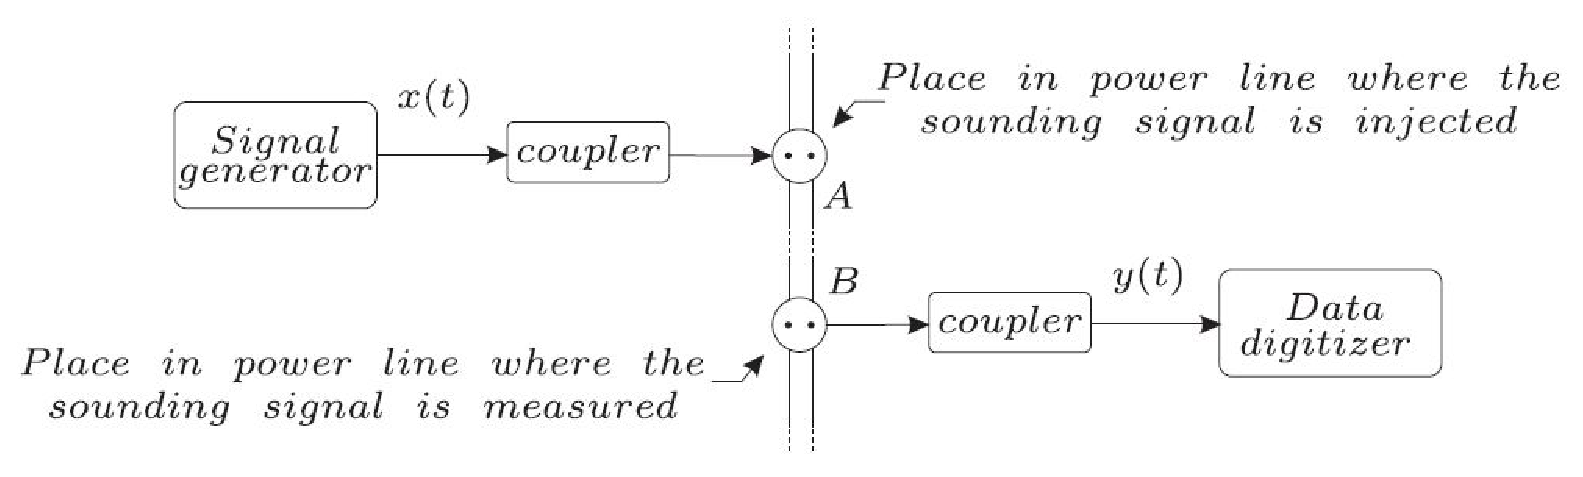
\includegraphics[width=0.9\textwidth]{images/PLC_measurement_setup.eps}
	\caption{Block diagram of the PLC measurement setup.}
	\label{fig_setup_PLC}
\end{figure}

From the entire campaign, $245$ different combinations of pairs of outlets were measured, providing a total of $148,037$ different \ac{CFR} estimates, with an average of $604$ consecutive \ac{CFR} estimates for each \ac{PLC} channel configuration. 

\begin{table}[h]
	\setlength\extrarowheight{4.5pt}
	\centering
	\caption{Characteristics of the measured residences.}
	\label{table_ap}
	\resizebox{0.9\textwidth}{!}{%
		\begin{tabular}{|C{3.75cm}|C{2.8cm}|C{4.5cm}|C{3.75cm}|}%{@{ }|c|c|c|c|@{ }}
			\cline{1-4}
			%\toprule
			Construction Type & Age (years) & Constructed area ($m^2$) & Considered Outlets \\ \cline{1-4}%\midrule
			House \# 1        & 30          & 78                       & 12                 \\
			House \# 2        & 10          & 69                       & 14                 \\
			Apartment \# 1    & 9           & 54                       & 11                 \\
			Apartment \# 2    & 9           & 42                       & 06                 \\
			Apartment \# 3    & 19          & 65                       & 11                 \\
			Apartment \# 4    & 3           & 62                       & 11                 \\
			Apartment \# 5    & 2           & 54                       & 11                 \\ \cline{1-4}%\bottomrule
		\end{tabular}%
	}
\end{table}

The \ac{CFR} measurement setup used for acquiring the estimations of hybrid \ac{PLC}-wireless \acp{CFR}, is illustrated in Fig. \ref{fig_setup_Hybrid}. These measurements were carried out in the residences listed in Table \ref{table_ap}, potential scattering objects and the transceivers were stationary during the measurement campaign in order to avoid Doppler effects in the wireless portion of the hybrid \ac{PLC}-wireless channel. The hybrid-\ac{PLC} and hybrid-wireless transceivers are rugged computers equipped with a high-speed data acquisition board and a high-speed arbitrary signal generation board that operate as receiver and transmitter, respectively. The coupler is the same circuitry used in the \ac{PLC} measurement setup with the objective of blocking the main voltage signal and presenting very low attenuations in the bandwidth of interest. The adopted omnidirectional and monopole antenna operate in the frequency band ranging from $1$~MHz up to $1$~GHz.

\begin{figure}[h]
	\centering
	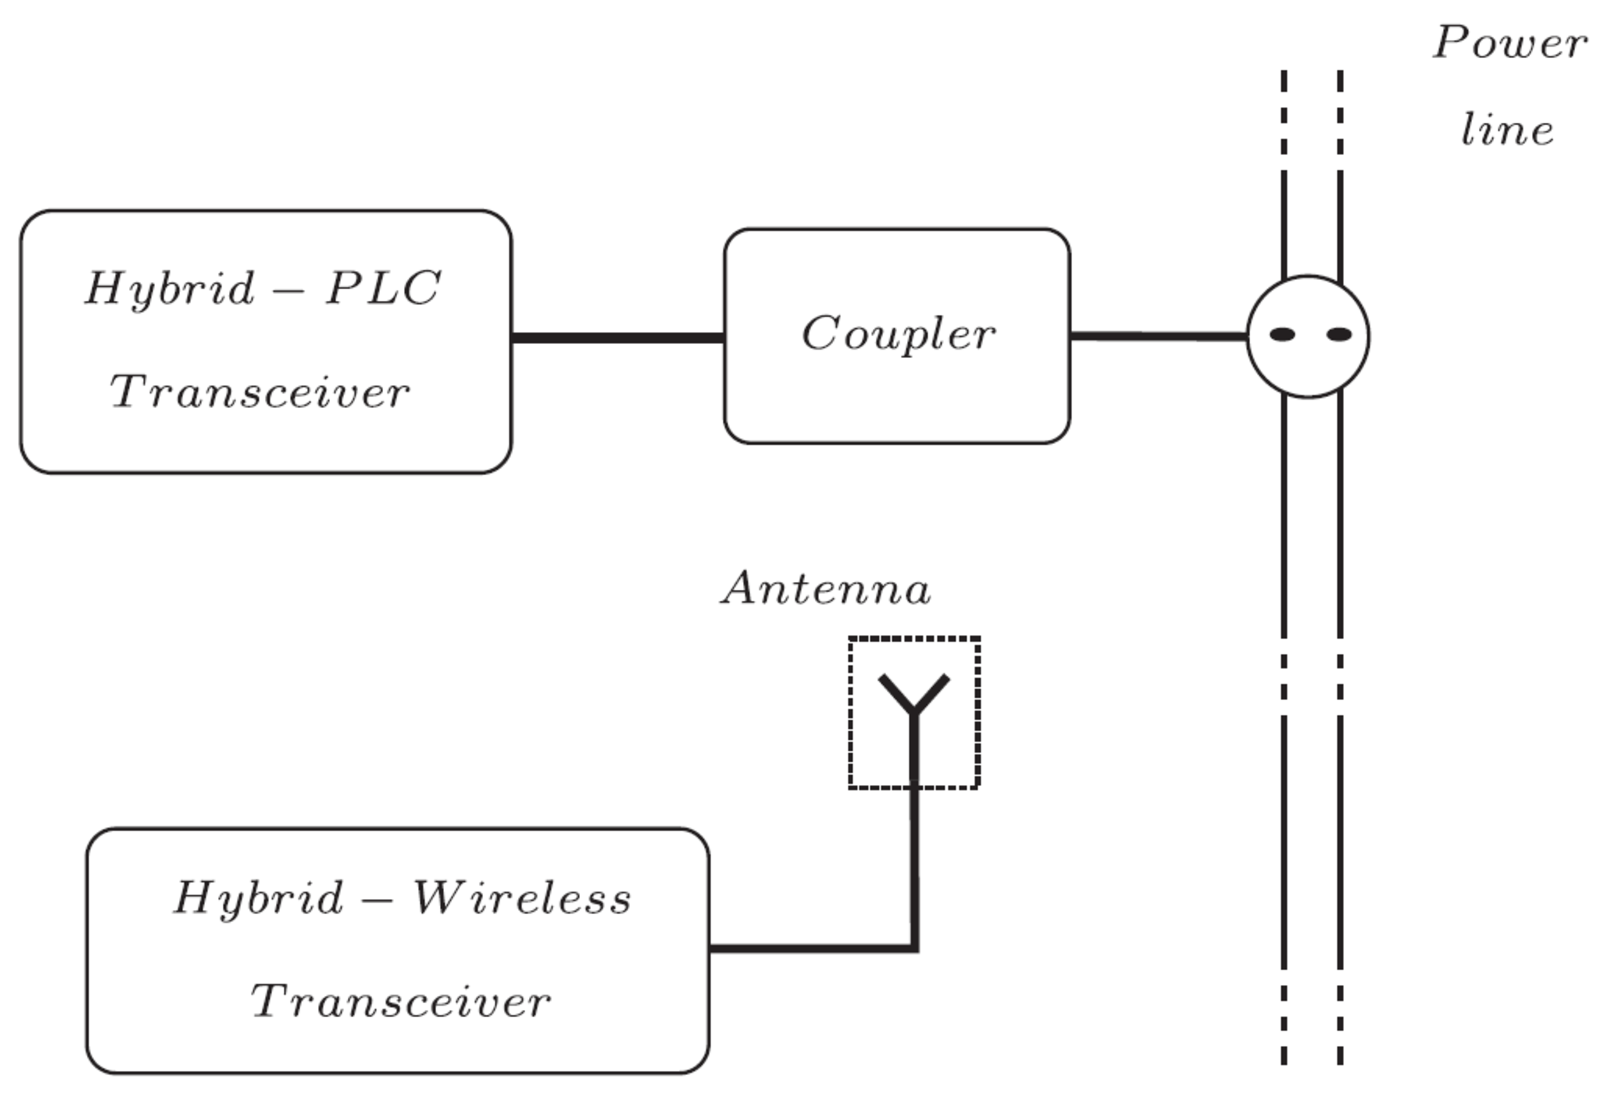
\includegraphics[width=0.65\textwidth]{images/Hybrid_measurement_setup.eps}
	\caption{Block diagram of the hybrid PLC-wireless measurement setup.}
	\label{fig_setup_Hybrid}
\end{figure}

By taking into account all facilities, $293$ different combinations of locations for both transceivers were evaluated. The hybrid-wireless transceiver was positioned near to (\textit{short-path channel}) and far from (\textit{long-path channel}) the outlet in $200$ and $93$ combinations, respectively. Furthermore, an average of 600 estimates of \acp{CFR} were measured for each combination, resulting on a total of $175,428$ different estimates of the hybrid \ac{PLC}-wireless channel frequency responses, obtained during the campaign.

\chapter{In-home PLC channels in the frequency band delimited by $1.7$ and $100$~MHz: Tables of the values of cubic splines used to model the parameter of the Beta Distribution.} \label{ap:c}

\begin{table*}[h]
	\setlength\extrarowheight{4.5pt}
	\centering
	\caption{$\alpha(f)$ parameter: Coefficients of the cubic Splines for $L=19$ nonuniform subbands.}
	\label{table_alfa}
	\begin{tabular}{|C{4cm}|C{2.7cm}|C{2.7cm}|C{2.7cm}|C{2.7cm}|m{0cm}}
		\cline{1-5}
		Frequency Band (MHz)           		   & $a_u$    			  & $b_u$      			 & $c_u$   		 		& $d_u$&\\ \cline{1-5}
		$1.70\textless \mid f\mid \leq 3.42$   & -2.6528 $\times 10^{-5}$ & 0.0033  				 & -0.1197 					& 2.5007 &\\ \cline{1-5}
		$3.42\textless \mid f\mid \leq 4.44$   & -2.6528 $\times 10^{-5}$ & 5.2561 $\times 10^{-4}$  & 0.0146  					& 1.2292 &\\ \cline{1-5}
		$4.44\textless \mid f\mid \leq 6.05$   & 1.7869  $\times 10^{-5}$ & -0.0011                  & 0.0015                   & 1.5211 &\\ \cline{1-5}
		$6.05\textless \mid f\mid \leq 8.50$   & -5.9605 $\times 10^{-6}$ & 6.2337 $\times 10^{-4}$  & -0.0157                  & 0.9666 &\\ \cline{1-5}
		$8.50\textless \mid f\mid \leq 12.01$  & 2.0887  $\times 10^{-6}$ & -2.7071 $\times 10^{-4}$ & 0.0019 					& 0.9954 &\\ \cline{1-5}
		$12.01\textless \mid f\mid \leq 17.19$ & -9.2474 $\times 10^{-7}$ & 1.8046 $\times 10^{-4}$  & -0.0046 					& 0.5114 &\\ \cline{1-5}
		$17.19\textless \mid f\mid \leq 22.36$ & 6.4104  $\times 10^{-7}$ & -1.1361 $\times 10^{-4}$ & 0.0025  					& 0.9547 &\\ \cline{1-5}
		$22.36\textless \mid f\mid \leq 27.53$ & -5.6131 $\times 10^{-7}$ & 9.0243 $\times 10^{-5}$  & 5.3515 $\times 10^{-5}$  & 0.7099 &\\ \cline{1-5}
		$27.53\textless \mid f\mid \leq 32.71$ & 4.7371  $\times 10^{-7}$ & -8.8254 $\times 10^{-5}$ & -2.6432 $\times 10^{-4}$ & 1.0610 &\\ \cline{1-5}
		$32.71\textless \mid f\mid \leq 43.06$ & -1.7026 $\times 10^{-7}$ & 6.2385 $\times 10^{-5}$  & -0.0025 					& 0.6616 &\\ \cline{1-5}
		$43.06\textless \mid f\mid \leq 48.24$ & 1.4089  $\times 10^{-7}$ & -4.5902 $\times 10^{-5}$ & 0.0010  					& 1.3178 &\\ \cline{1-5}
		$48.24\textless \mid f\mid \leq 53.42$ & 1.4415  $\times 10^{-7}$ & -1.0984 $\times 10^{-6}$ & -0.0040 					& 1.0777 &\\ \cline{1-5}
		$53.42\textless \mid f\mid \leq 58.60$ & -2.7951 $\times 10^{-7}$ & 4.4742 $\times 10^{-5}$  & 6.6073 $\times 10^{-4}$  & 0.8167 &\\ \cline{1-5}
		$58.60\textless \mid f\mid \leq 68.95$ & 1.4642  $\times 10^{-7}$ & -4.4142 $\times 10^{-5}$ & 7.2426 $\times 10^{-4}$  & 1.0565 &\\ \cline{1-5}
		$68.95\textless \mid f\mid \leq 74.12$ & -3.5410 $\times 10^{-7}$ & 4.8981 $\times 10^{-5}$  & 0.0018 					& 0.6212 &\\ \cline{1-5}
		$74.12\textless \mid f\mid \leq 79.30$ & 4.3096  $\times 10^{-7}$ & -6.3623 $\times 10^{-5}$ & 1.9804 $\times 10^{-4}$  & 0.9354 &\\ \cline{1-5}
		$79.30\textless \mid f\mid \leq 84.47$ & -3.8389 $\times 10^{-7}$ & 7.3423 $\times 10^{-5}$  & 0.0012					& 0.7548 &\\ \cline{1-5}
		$84.47\textless \mid f\mid \leq 94.82$ & 9.4613 $\times 10^{-8}$  & -4.8652 $\times 10^{-5}$ & 0.0039 					& 1.2537 &\\ \cline{1-5}
		$94.82\textless \mid f\mid \leq 100$   & 9.4613  $\times 10^{-8}$ & 1.1522 $\times 10^{-5}$  & -0.0040					& 0.7874 &\\ \cline{1-5}
	\end{tabular}
\end{table*}

\begin{table*}[h]
	\setlength\extrarowheight{4.5pt}
	\centering
	\caption{$\beta(f)$ parameter: Coefficients of the cubic Splines for $L=19$ nonuniform subbands.}
	\label{table_beta}
	\begin{tabular}{|C{4cm}|C{2.7cm}|C{2.7cm}|C{2.7cm}|C{2.7cm}|m{0cm}}
		\cline{1-5}
		Frequency Band (MHz)           		   & $a_u$    			   & $b_u$      			  & $c_u$   		 		& $d_u$ &\\ \cline{1-5}
		$1.70\textless \mid f\mid \leq 3.42$   & 0 						   & 0.0112 				  & -0.3463 				& 5.1804  &\\ \cline{1-5}
		$3.42\textless \mid f\mid \leq 4.44$   & -9.0897 $\times 10^{-5}$  & 0.0016 				  & 0.1020  				& 2.8535  &\\ \cline{1-5}
		$4.44\textless \mid f\mid \leq 6.05$   & 6.0160  $\times 10^{-5}$  & -0.0041 				  & 0.0503 					& 4.8733  &\\ \cline{1-5}
		$6.05\textless \mid f\mid \leq 8.50$   & -1.9159 $\times 10^{-5}$  & 0.0019 				  & -0.0234 				& 4.2359  &\\ \cline{1-5}
		$8.50\textless \mid f\mid \leq 12.01$  & 7.2688  $\times 10^{-6}$  & -0.0010 				  & 0.0191 					& 5.3245  &\\ \cline{1-5}
		$12.01\textless \mid f\mid \leq 17.19$ & -3.1854 $\times 10^{-6}$  & 5.5773 $\times 10^{-4}$  & -0.0137 				& 4.1615  &\\ \cline{1-5}
		$17.19\textless \mid f\mid \leq 22.36$ & 3.4012 $\times 10^{-6}$   & -4.5522 $\times 10^{-4}$ & -0.0028  				& 5.1844  &\\ \cline{1-5}
		$22.36\textless \mid f\mid \leq 27.53$ & -3.4336 $\times 10^{-6}$  & 6.2635 $\times 10^{-4}$  & 0.0153 					& 3.8223  &\\ \cline{1-5}
		$27.53\textless \mid f\mid \leq 32.71$ & 1.8876  $\times 10^{-6}$  & -4.6554 $\times 10^{-4}$ & 0.0324 					& 8.3953  &\\ \cline{1-5}
		$32.71\textless \mid f\mid \leq 43.06$ & -2.0279 $\times 10^{-7}$  & 1.3472 $\times 10^{-4}$  & -0.0027 				& 8.8443  &\\ \cline{1-5}
		$43.06\textless \mid f\mid \leq 48.24$ & -1.1405  $\times 10^{-6}$ & 5.7440 $\times 10^{-6}$  & 0.0271  				& 12.3956 &\\ \cline{1-5}
		$48.24\textless \mid f\mid \leq 53.42$ & 2.6168  $\times 10^{-6}$  & -3.5693 $\times 10^{-4}$ & -0101 					& 13.9729 &\\ \cline{1-5}
		$53.42\textless \mid f\mid \leq 58.60$ & -2.6679 $\times 10^{-6}$  & 4.7522 $\times 10^{-4}$  & 0.0024 					& 12.0045 &\\ \cline{1-5}
		$58.60\textless \mid f\mid \leq 68.95$ & 1.4275  $\times 10^{-6}$  & -3.7318 $\times 10^{-4}$ & 0.0132 					& 14.4208 &\\ \cline{1-5}
		$68.95\textless \mid f\mid \leq 74.12$ & -4.7854 $\times 10^{-6}$  & 5.3473 $\times 10^{-4}$  & 0.0475 					& 14.0510 &\\ \cline{1-5}
		$74.12\textless \mid f\mid \leq 79.30$ & 8.4579  $\times 10^{-6}$  & -9.8702 $\times 10^{-4}$ & -4.8272 $\times 10^{-4}$& 19.3107 &\\ \cline{1-5}
		$79.30\textless \mid f\mid \leq 84.47$ & -9.4143 $\times 10^{-6}$  & 0.0017 				  & 0.0754 					& 18.3228 &\\ \cline{1-5}
		$84.47\textless \mid f\mid \leq 94.82$ & 3.5082 $\times 10^{-6}$   & -0.0013 				  & 0.1190					& 34.2297 &\\ \cline{1-5}
		$94.82\textless \mid f\mid \leq 100$   & 3.5082 $\times 10^{-6}$   & 9.4005 $\times 10^{-4}$  & 0.0445 					& 34.8507 &\\ \cline{1-5}
	\end{tabular}
\end{table*}

\chapter{In-home hybrid PLC-WLC \textit{short-path} channels in the frequency band delimited by $1.7$ and $100$~MHz: Tables of the values of cubic splines used to model the parameters of the Log-Normal Distribution.} \label{ap:e}

\begin{table}[h]
	\setlength\extrarowheight{4.5pt}
	\centering
	\caption{$\mu(f)$ parameter: Coefficients of the cubic Splines for  $L=15$  nonuniform subbands.}
	\label{table_alfasW}
	\begin{tabular}{|C{4cm}|C{2.7cm}|C{2.7cm}|C{2.7cm}|C{2.7cm}|m{0cm}}
		\cline{1-5}
		Frequency Band (MHz)           		   & $a_u$    			  	  & $b_u$	      			  & $c_u$  	 		 		 & $d_u$&\\ \cline{1-5}
		$1.70\textless \mid f\mid \leq 5.08$   & 2.3701  $\times 10^{-6}$ & -6.0903 $\times 10^{-4}$  & 0.0500 					 & -7.9514 &\\ \cline{1-5}
		$5.08\textless \mid f\mid \leq 6.54$   & 2.3701  $\times 10^{-6}$ & -1.1842 $\times 10^{-4}$  & -1.7145 $\times 10^{-4}$ & -6.6209 &\\ \cline{1-5}
		$6.54\textless \mid f\mid \leq 8.50$   & 3.9289  $\times 10^{-6}$ & 9.4894  $\times 10^{-5}$  & -8.7708 $\times 10^{-4}$ & -6.6686 &\\ \cline{1-5}
		$8.50\textless \mid f\mid \leq 9.47$   & -1.7588 $\times 10^{-5}$ & 5.6636  $\times 10^{-4}$  & 0.0256                   & -6.3004 &\\ \cline{1-5}
		$9.47\textless \mid f\mid \leq 13.87$  & 2.4037  $\times 10^{-6}$ & -4.8890 $\times 10^{-4}$  & 0.0271					 & -5.7031 &\\ \cline{1-5}
		$13.87\textless \mid f\mid \leq 21.19$ & -5.6687 $\times 10^{-7}$ & 1.6009  $\times 10^{-4}$  & -0.0025		    		 & -5.4699 &\\ \cline{1-5}
		$21.19\textless \mid f\mid \leq 28.03$ & 3.7473  $\times 10^{-7}$ & -9.4996 $\times 10^{-5}$  & 0.0073  				 & -4.1516 &\\ \cline{1-5}
		$28.03\textless \mid f\mid \leq 33.40$ & -3.4080 $\times 10^{-7}$ & 6.2389  $\times 10^{-5}$  & 0.0027 					 & -3.9641 &\\ \cline{1-5}
		$33.40\textless \mid f\mid \leq 43.46$ & 1.0904  $\times 10^{-7}$ & -5.0076 $\times 10^{-5}$  & 0.0041  				 & -3.3626 &\\ \cline{1-5}
		$43.46\textless \mid f\mid \leq 50.49$ & -8.8509 $\times 10^{-8}$ & 1.7312  $\times 10^{-5}$  & -0.0027					 & -3.6932 &\\ \cline{1-5}
		$50.49\textless \mid f\mid \leq 55.37$ & 1.2130  $\times 10^{-7}$ & -2.0924 $\times 10^{-5}$  & -0.0032  				 & -3.9824 &\\ \cline{1-5}
		$55.37\textless \mid f\mid \leq 65.14$ & -3.1804 $\times 10^{-8}$ & 1.5465  $\times 10^{-5}$  & -0.0037 				 & -4.3889 &\\ \cline{1-5}
		$65.14\textless \mid f\mid \leq 74.90$ & 1.7372  $\times 10^{-8}$ & -3.6169 $\times 10^{-6}$  & -0.0014  			     & -4.7710 &\\ \cline{1-5}
		$74.90\textless \mid f\mid \leq 96.87$ & -1.2395 $\times 10^{-8}$ & 6.8061  $\times 10^{-6}$  & -7.2408 $\times 10^{-4}$ & -5.0491 &\\ \cline{1-5}
		$96.87\textless \mid f\mid \leq 100$   & -1.2395 $\times 10^{-8}$ & -9.9272 $\times 10^{-6}$  & -0.0021 				 & -5.1262 &\\ \cline{1-5}
	\end{tabular}
\end{table}

\begin{table*}[h]
	\setlength\extrarowheight{4.5pt}
	\centering
	\caption{$\sigma(f)$ parameter: Coefficients of the cubic Splines for the $L=15$ nonuniform subbands.}
	\label{table_betasW}
	\begin{tabular}{|C{4cm}|C{2.7cm}|C{2.7cm}|C{2.7cm}|C{2.7cm}|m{0cm}}
		\cline{1-5}
		Frequency Band (MHz)           		   & $a_u$    			   	   & $b_u$      			  & $c_u$   		 		 & $d_u$ &\\ \cline{1-5}
		$1.70\textless \mid f\mid \leq 2.88$   & 2.1232 $\times 10^{-5}$   & -0.0021 				  & 0.0435	 				 & 1.2187 &\\ \cline{1-5}
		$2.88\textless \mid f\mid \leq 4.35$   & 2.1232 $\times 10^{-5}$   & -5.2494 $\times 10^{-4}$ & -0.0184  				 & 1.3724 &\\ \cline{1-5}
		$4.35\textless \mid f\mid \leq 5.08$   & -5.8155 $\times 10^{-5}$  & 0.0014 				  & 0.0074 					 & 0.9206 &\\ \cline{1-5}
		$5.08\textless \mid f\mid \leq 6.54$   & 2.0568 $\times 10^{-5}$   & -0.0012 				  & 0.0097	 				 & 1.1473 &\\ \cline{1-5}
		$6.54\textless \mid f\mid \leq 8.50$   & -8.0700 $\times 10^{-6}$  & 6.2010 $\times 10^{-4}$  & -0.0086 				 & 0.8867 &\\ \cline{1-5}
		$8.50\textless \mid f\mid \leq 10.69$  & 3.7423 $\times 10^{-6}$   & -3.4830 $\times 10^{-4}$ & 0.0023	 				 & 1.0186 &\\ \cline{1-5}
		$10.69\textless \mid f\mid \leq 17.28$ & -6.3590 $\times 10^{-7}$  & 1.5692 $\times 10^{-4}$  & -0.0063  				 & 0.7568 &\\ \cline{1-5}
		$17.28\textless \mid f\mid \leq 22.66$ & 4.4496 $\times 10^{-7}$   & -1.0063 $\times 10^{-4}$ & 0.0013 					 & 1.1968 &\\ \cline{1-5}
		$22.66\textless \mid f\mid \leq 35.06$ & -1.0044  $\times 10^{-7}$ & 4.6212 $\times 10^{-5}$  & -0.0047					 & 0.7106 &\\ \cline{1-5}
		$35.06\textless \mid f\mid \leq 39.84$ & 1.5003  $\times 10^{-7}$  & -3.0325 $\times 10^{-5}$ & -6.8556 $\times 10^{-4}$ & 0.8469 &\\ \cline{1-5}
		$39.84\textless \mid f\mid \leq 60.25$ & -1.8796 $\times 10^{-8}$  & 1.3785  $\times 10^{-5}$ & -0.0023  				 & 0.6297 &\\ \cline{1-5}
		$60.25\textless \mid f\mid \leq 68.55$ & 1.2989   $\times 10^{-7}$ & -9.7855 $\times 10^{-6}$ & -6.3475	$\times 10^{-4}$ & 0.7014 &\\ \cline{1-5}
		$78.61\textless \mid f\mid \leq 78.61$ & -2.1013 $\times 10^{-7}$  & 2.9181  $\times 10^{-5}$ & 0.0013					 & 0.6699 &\\ \cline{1-5}
		$78.61\textless \mid f\mid \leq 94.43$ & 2.2893  $\times 10^{-8}$  & -1.4947 $\times 10^{-5}$ & 0.0023				     & 0.8322 &\\ \cline{1-5}
		$94.43\textless \mid f\mid \leq 100$   & 1.0785  $\times 10^{-8}$  & -5.2390 $\times 10^{-7}$ & -9.4771 $\times 10^{-4}$ & 0.8683 &\\ \cline{1-5}
	\end{tabular}
\end{table*}

\chapter{In-home hybrid PLC-WLC \textit{long-path} channels in the frequency band delimited by $1.7$ and $100$~MHz: Tables of the values of cubic splines used to model the parameters of the Log-Normal Distribution.} \label{ap:g}

\begin{table*}[h]
	\setlength\extrarowheight{4.5pt}
	\centering
	\caption{$\mu(f)$ parameter: Coefficients of the cubic Splines for $L=15$ nonuniform subbands.}
	\label{table_alfalW}
	\begin{tabular}{|C{4cm}|C{2.7cm}|C{2.7cm}|C{2.7cm}|C{2.7cm}|m{0cm}}
		\cline{1-5}
		Frequency Band (MHz)           		   & $a_u$    			   	   & $b_u$      			  & $c_u$   		 		 & $d_u$ &\\ \cline{1-5}
		$1.70\textless \mid f\mid \leq 6.44$   & -1.1271 $\times 10^{-6}$  & 1.7728 $\times 10^{-4}$  & 0.0026	 				 & -8.4445 &\\ \cline{1-5}
		$6.44\textless \mid f\mid \leq 14.84$  & -1.1271 $\times 10^{-6}$  & -1.2068 $\times 10^{-5}$ & 0.0119  				 & -7.9388 &\\ \cline{1-5}
		$14.84\textless \mid f\mid \leq 22.41$ & 1.1653  $\times 10^{-6}$  & -1.1350 $\times 10^{-4}$ & 0.0081 					 & -7.6235 &\\ \cline{1-5}
		$22.41\textless \mid f\mid \leq 25.59$ & -4.1434 $\times 10^{-6}$  & 2.1163 $\times 10^{-4}$  & 0.0172	 				 & -6.9126 &\\ \cline{1-5}
		$25.59\textless \mid f\mid \leq 27.69$ & 4.1926 $\times 10^{-6}$   & -4.3475 $\times 10^{-4}$ & 0.0056					 & -6.0262 &\\ \cline{1-5}
		$27.69\textless \mid f\mid \leq 32.57$ & -1.4955 $\times 10^{-6}$  & 2.5704 $\times 10^{-4}$  & -0.0041	 				 & -6.3333 &\\ \cline{1-5}
		$32.57\textless \mid f\mid \leq 33.40$ & 3.1809 $\times 10^{-7}$   & -9.2908 $\times 10^{-5}$ & 0.0087   				 & -5.8014 &\\ \cline{1-5}
		$33.40\textless \mid f\mid \leq 40.38$ & -2.6103 $\times 10^{-7}$  & 6.4547 $\times 10^{-5}$  & 0.0040 					 & -5.4711 &\\ \cline{1-5}
		$40.38\textless \mid f\mid \leq 44.04$ & 1.2268  $\times 10^{-7}$  & -6.8577 $\times 10^{-5}$ & 0.0033					 & -4.2094 &\\ \cline{1-5}
		$44.04\textless \mid f\mid \leq 48.24$ & -4.0204 $\times 10^{-8}$  & 2.4906 $\times 10^{-5}$  & -0.0078	 				 & -5.7833 &\\ \cline{1-5}
		$48.24\textless \mid f\mid \leq 57.81$ & 1.8952  $\times 10^{-8}$  & -6.6395 $\times 10^{-7}$ & -0.0026  				 & -6.6975 &\\ \cline{1-5}
		$57.81\textless \mid f\mid \leq 60.74$ & -2.8253  $\times 10^{-8}$ & 1.1389 $\times 10^{-5}$  & -3.7214 $\times 10^{-4}$ & -7.1077 &\\ \cline{1-5}
		$60.74\textless \mid f\mid \leq 68.94$ & 6.8867 $\times 10^{-8}$   & -6.5792 $\times 10^{-6}$ & 6.4762	$\times 10^{-4}$ & -6.9439 &\\ \cline{1-5}
		$68.94\textless \mid f\mid \leq 86.18$ & -5.6494  $\times 10^{-8}$ & 1.5321 $\times 10^{-5}$  & 0.0016 				     & -6.8672 &\\ \cline{1-5}
		$86.18\textless \mid f\mid \leq 100$   & -5.6494 $\times 10^{-8}$  & -1.7390 $\times 10^{-5}$ & 0.0012  				 & -6.3988 &\\ \cline{1-5}
	\end{tabular}
\end{table*}

\begin{table*}[h]
	\setlength\extrarowheight{4.5pt}
	\centering
	\caption{$\sigma(f)$ parameter: Coefficients of the cubic Splines for the $L=15$ nonuniform subbands.}
	\label{table_betalW}
	\begin{tabular}{|C{4cm}|C{2.7cm}|C{2.7cm}|C{2.7cm}|C{2.7cm}|m{0cm}}
		\cline{1-5}
		Frequency Band (MHz)           		   & $a_u$    			   	   & $b_u$      			  & $c_u$   		 		 & $d_u$ &\\ \cline{1-5}
		$1.70\textless \mid f\mid \leq 4.44$   & 1.3148  $\times 10^{-7}$  & -5.6568 $\times 10^{-5}$ & 0.0030	 				 & 1.4384 &\\ \cline{1-5}
		$4.44\textless \mid f\mid \leq 5.91$   & 1.3148  $\times 10^{-7}$  & -1.8306 $\times 10^{-5}$ & -0.0043  				 & 1.3175 &\\ \cline{1-5}
		$5.91\textless \mid f\mid \leq 10.45$  & -2.6464 $\times 10^{-7}$  & 4.9539 $\times 10^{-5}$  & 0.0011					 & 0.7124 &\\ \cline{1-5}
		$10.45\textless \mid f\mid \leq 12.99$ & 1.0831  $\times 10^{-6}$  & -7.3521 $\times 10^{-5}$ & -0.0026	 				 & 1.0896 &\\ \cline{1-5}
		$12.99\textless \mid f\mid \leq 15.68$ & -2.0515 $\times 10^{-6}$  & 1.3768  $\times 10^{-4}$ & 0.0016  				 & 0.9071 &\\ \cline{1-5}
		$15.68\textless \mid f\mid \leq 19.48$ & 8.9917 $\times 10^{-7}$   & -1.2695 $\times 10^{-4}$ & 0.0020	 				 & 1.0660 &\\ \cline{1-5}
		$19.48\textless \mid f\mid \leq 27.54$ & -4.7172 $\times 10^{-6}$  & 1.4280 $\times 10^{-4}$  & 0.0036 					 & 0.8984 &\\ \cline{1-5}
		$27.54\textless \mid f\mid \leq 35.84$ & 3.8415  $\times 10^{-7}$  & -9.7780 $\times 10^{-5}$ & 0.0044 					 & 0.9779 &\\ \cline{1-5}
		$35.84\textless \mid f\mid \leq 48.24$ & -5.4667 $\times 10^{-7}$  & 6.7022 $\times 10^{-5}$  & -2.1365	$\times 10^{-5}$ & 0.7276 &\\ \cline{1-5}
		$48.24\textless \mid f\mid \leq 58.59$ & 3.4176  $\times 10^{-7}$  & -5.5979 $\times 10^{-5}$ & 8.0683	$\times 10^{-4}$ & 0.8724 &\\ \cline{1-5}
		$58.59\textless \mid f\mid \leq 68.94$ & -1.0467 $\times 10^{-7}$  & 3.2196 $\times 10^{-5}$  & -0.0012  				 & 0.7451 &\\ \cline{1-5}
		$68.94\textless \mid f\mid \leq 79.30$ & 2.4291  $\times 10^{-7}$  & -2.9349 $\times 10^{-5}$ & -6.8042	$\times 10^{-4}$ & 0.9511 &\\ \cline{1-5}
		$79.30\textless \mid f\mid \leq 84.47$ & -3.2976 $\times 10^{-8}$  & 1.4375 $\times 10^{-5}$  & -0.0016  				 & 0.8571 &\\ \cline{1-5}
		$84.47\textless \mid f\mid \leq 93.90$ & 2.9498  $\times 10^{-9}$  & -2.2454 $\times 10^{-6}$ & 4.5886	$\times 10^{-4}$ & 0.8412 &\\ \cline{1-5}
		$93.90\textless \mid f\mid \leq 100$   & 2.9498  $\times 10^{-9}$  & 8.7842 $\times 10^{-7}$  & -2.3694 $\times 10^{-5}$ & 0.8531 &\\ \cline{1-5}
	\end{tabular}
\end{table*}

\chapter{List of Publications} \label{ap:i}

The list of journal papers published or submitted during the graduate period is as follows:

\begin{itemize}
	\item T. F. do A. Nogueira, G. R. Colen, V. Fernandes and M. V. Ribeiro, ``Statistical Characterization and Modelings of Frequency Responses of Brazilian In-Home PLC Channels,'' in \textit{IEEE System Journal}, under review.
\end{itemize}

\begin{itemize}
	\item V. Fernandes, T. F. do A. Nogueira, H. V. Poor and M. V. Ribeiro, ``Statistical Modeling for Dedicated Energy Harvesting in Hybrid PLC-Wireless Channels,'' in \textit{IEEE Trans. on Smart Grid}, submitted.
\end{itemize}


